\chapter{Teoria}

Kluczowym aspektem pracy, na której bazuje duża część funkcjonalności jest model uczenia maszynowego oparty na architekturze transformerów. 
Przy jego pomocy aplikacja będzie w stanie rozpoznawać znaki języka migowego w czasie rzeczywistym.
Transformery stanowią szczególną część szeroko pojętej dziedziny uczenia maszynowego, znajdują one zastosowanie w przetwarzaniu języka naturalnego, wizji komputerowej, ale~także w audio i~przetwarzaniu multimedialnym. \\
W odróżnieniu od poprzednio stosowanych modeli uczenia maszynowego opierających się na podejściu rekurencyjnym i mechanizmie uwagi, naukowcy pracujący dla firmy Google zaproponowali rozwiązanie wykorzystujące jedynie mechanizm uwagi. 
Jest to istotny element, który róznicuje transformery od rekurencyjnych modeli uczenia maszynowego.
Wyzbycie się rekurencyjności w procesie uczenia przyczyniło się do zwiększenia równoległości, skutkiem czego jest znaczne przyspieszenie czasu uczenia modelu przy zachowaniu wysokiej precyzji \cite{vaswani2023attentionneed}.

W tradycyjnych modelach rekurencyjnych sieci neuronowych (RNN) dane przetwarzane są sekwencyjnie tzn., że są analizowane krok po kroku (patrz \ref{fig:rnn_schema}) \cite{mamczur2020} co skutkuje ograniczeniami m.in. w równoległości przetwarzaniu danych.


\begin{figure}[H]
    \centering
	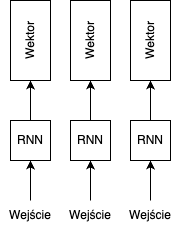
\includegraphics[scale=0.60]{figs/rnn.png}
	\caption{Przepływ informacji wejściowych w rekurencyjnych sieciach neuronowych}
	\label{fig:rnn_schema}
\end{figure}

Rozwiązania inżynieryjne wykorzystane w transformerach pozwalają modelom na przetwarzanie wszystkich elementów sekwencji jednocześnie (patrz \ref{fig:transformer_schema}).

\begin{figure}[H]
    \centering
	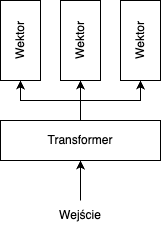
\includegraphics[scale=0.60]{figs/transformer.png}
	\caption{Przepływ informacji wejściowych w transformerach}
	\label{fig:transformer_schema}
\end{figure}

W praktyce oznacza to, że uczenie transformerów przebiega w określonej stałej ilości $O(1)$ sekwencyjnie wykonywanych operacji, modele RNN wymagają natomiast $O(n)$ sekwencyjnie wykonywanych operacji. %co sprawia, że są mniej wydajne przy dłuższych sekwencjach. 
% Autorzy uzasadniają wybór mechanizmu samo-uwagi ponad znane już sieci konwolucyjne oraz sieci rekurencyjne faktem iz złożoność obliczeniowa dla poszczególnych warstw jest mniejsza, a wiele operacji wykonywanych podczas trenowania modelu mozna zrownoleglic.
% Dodatkowo odległości pomiędzy zależnościami 

% The third is the path length between long-range dependencies in the network. Learning long-range
% dependencies is a key challenge in many sequence transduction tasks. 
% One key factor affecting the
% ability to learn such dependencies is the length of the paths forward and backward signals have to
% traverse in the network. 
% The shorter these paths between any combination of positions in the input
% and output sequences, the easier it is to learn long-range dependencies [12]. 
% Hence we also compare
% the maximum path length between any two input and output positions in networks composed of the
% different layer types.

\section{Architektura}

Na architekturę transformera składają się dwa główne komponenty: koder oraz dekoder. %, natomiast najpierw 

Koder składa się z warstwy osadzeń (eng. embedding layer) oraz kodowania pozycyjnego, po których następuje wiele warstw kodera.
Warstwa osadzeń zamienia dane wejściowe (słowa, obrazy) na ich reprezentacje w postaci wektorów.
Zazwyczaj reprezentacja jest wektorem o wartości rzeczywistej, który koduje znaczenie słowa w taki sposób, że oczekuje się, że słowa znajdujące się bliżej w przestrzeni wektorowej będą miały podobne znaczenie \cite{jm3}.
Osadzanie słów można uzyskać za pomocą modelowania języka i technik uczenia się cech, w których słowa lub frazy ze słownictwa są mapowane na wektory liczb rzeczywistych.

W przypadku modeli Vision Transformer (ViT) proces osadzania obrazów wygląda inaczej niż w przypadku osadzania słów.
Obrazy są dzielone na małe, prostokątne fragmenty (eng. patches), które następnie przekształcane są na wektory.
Zatem zamiast słow przetwarzane są fragmenty obrazów które dodatkowo mają przypisaną pozycje co pozwala modelowi rozróżnić położenie każdego fragmentu w konteście całego obrazu.
W celu przeprowadzenia klasyfikacji jako parametr wejściowy sekwencji podaje się poza odpowiednio wydzielonymi fragmentami obrazu równiez ,,token klasyfikacyjny'' (eng. classification token).
Proces ten przedstawiono na schemacie \ref{fig:vit_scheme} \cite{DBLP:journals/corr/abs-2010-11929}, a struktura sieci transformerowej jak podnoszą autorzy jest mozliwie najblizsza do struktury zaprezentowanej w artykule ,,Attention is All You Need''.

\begin{figure}[H]
    \centering
	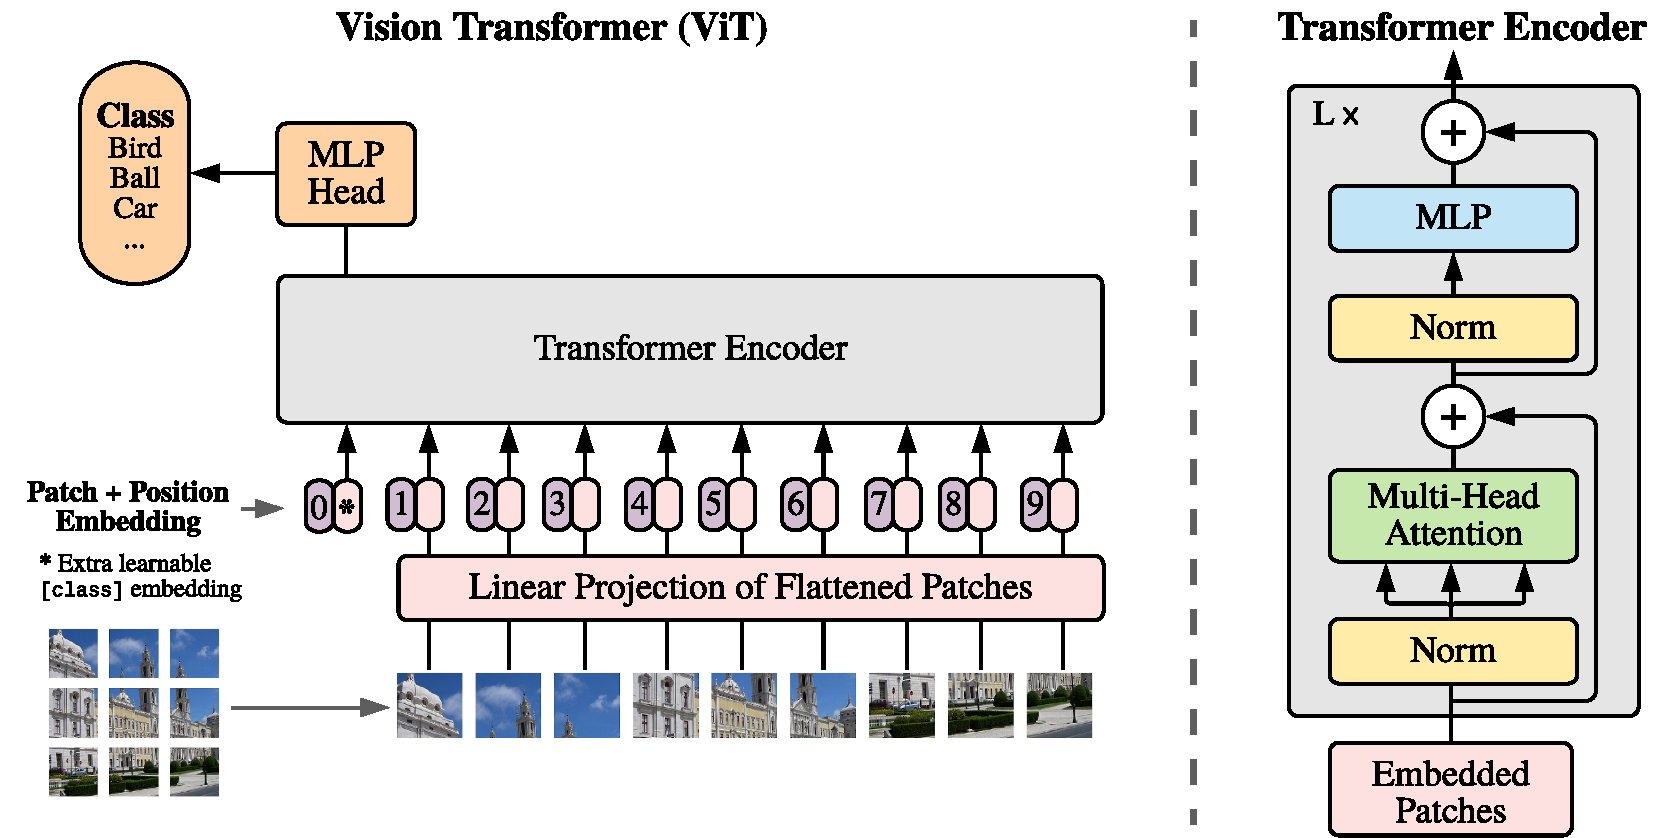
\includegraphics[scale=0.50]{figs/vit_scheme.pdf}
	\caption{Schemat uczenia modelu Transformer Vision}
	\label{fig:vit_scheme}
\end{figure}

Głównym zadaniem kodera jest przekształcanie wejściowych tokenów w kontekstowe reprezentacje. 
W przeciwieństwie do wcześniejszych modeli, które przetwarzały tokeny niezależnie, koder w transformerze przechwytuje kontekst każdego tokena w odniesieniu do całej sekwencji.
Ponieważ transformery nie mają mechanizmu rekurencji, takiego jak RNN, używają kodowania pozycyjnego dodanego do warstwy osadzeń w celu dostarczenia informacji o pozycji każdego tokena w sekwencji.
Każda z warstw kodera składa się z dwóch głownych komponentów: mechanizmu samo-uwagi i sieci neuronowej typu feed-forward. 
Koder pobiera dane wejściowe jako sekwencję wektorów wejściowych, stosuje mechanizm samo-uwagi aby utworzyć pośrednią sekwencję wektorów, a następnie stosuje warstwę feed-forward dla każdego wektora indywidualnie.
Warstwy kodera są ułożone w stos, gdzie pierwsza warstwa kodera pobiera sekwencję wektorów wejściowych z warstwy osadzania, tworząc sekwencję wektorów. 
Ta sekwencja wektorów jest przetwarzana przez drugi koder i tak dalej. 
Dane wyjściowe z ostatniej warstwy kodera są następnie wykorzystywane przez dekoder.

Dekoder podobnie do kodera, składa się z warstwy embedding layer oraz kodowania pozycyjnego, po której następuje wiele warstw dekodera.
Rola dekodera opiera się na tworzeniu sekwencji tekstowych.
Każdy dekoder składa się z trzech głównych elementów: maskowanego mechanizmu samo-uwagi, mechanizmu uwagi krzyżowej i sieci neuronowej typu feed-forward.
Dekoder działa w podobny sposób jak koder, ale wstawiony jest dodatkowy mechanizm uwagi, który zamiast tego czerpie istotne informacje z kodowań generowanych przez kodery. 
Mechanizm ten można również nazwać uwagą kodera-dekodera.
Podobnie jak pierwszy koder, pierwszy dekoder pobiera informacje pozycyjne i osadzenia sekwencji wyjściowej jako dane wejściowe, a nie kodowania.
Transformer nie może wykorzystywać bieżącego lub przyszłego wyjścia do przewidywania wyjścia, więc sekwencja wyjściowa musi być częściowo zamaskowana, aby zapobiec temu odwrotnemu przepływowi informacji. 
W przypadku dekodowania, uwaga all-to-all jest nieodpowiednia, ponieważ token nie może zwracać uwagi na tokeny, które nie zostały jeszcze wygenerowane.
W ten sposób moduł samo-uwagi w dekoderze jest przyczynowo maskowany.
W przeciwieństwie do tego, mechanizm uwagi krzyżowej zwraca uwagę na wektory wyjściowe kodera, które są obliczane przed rozpoczęciem dekodowania przez dekoder.
W związku z tym nie ma potrzeby maskowania w mechanizmie uwagi krzyżowej.

% Zanim dane przetwarzane przez transformer zostaną przekazane do kodera muszą zostać wstępnie przetworzone. Proces ten można podzielić na dwa kroki:
% \begin{itemize}
%     \item Input Embedding polega na zamienieniu danych wejściowych na przystępne dla obliczeń komputerowych wektory.
%     \item Positional Encoding składa się z wektorów, których zadaniem jest nadanie kontekstu na podstawie pozycji danych w sekwencji. Jest to istotne, gdyż z~punktu widzenia maszyny nie jest wstanie odróżnić ona informacji użytych w różnym znaczeniu. 
% \end{itemize}
% Sam koder składa się z dwóch elementów:
% \begin{itemize}
%     \item Multi-Head Attention polega na obliczeniu wektora uwagi dla poszczególnych informacji przekazanych do tej warstwy. W tym etapie obliczany jest tzw. wektor uwagi za pomocą którego określa się wagę poszczególnych informacji. W przypadku przetwarzania wideo identyfikowane są kluczowe momenty takie jak m.in. gesty poprzez nadanie wag poszczególnym klatkom wideo w zależności od ich znaczenia. Ignorowane są mniej istotne informacje lub szum.
%     \item Feed Forward, w tym etapie obliczone wektory przekazywane są do sieci MLP (Multi Layer Perceptron), która używana jest dla każdego wektora uwagi.
% \end{itemize}
% Tak przygotowane dane zostają przekazane do dekodera, którego zadaniem jest przewidywanie kolejnych słów czy obrazów. W tym procesie udział biorą poszczególne bloki:
% \begin{itemize}
%     \item Embedding proces ten przebiega dokładnie tak samo jak w przypadku warstwy kodującej. Dane zamieniane są na wartości numeryczne w postaci macierzy.
%     \item Positional Encoding również odbywa się w taki sam sposób jak w przypadku warstwy kodującej. Obliczane są wektory nadające kontekst informacjom.
%     \item Masked Multi-Head Attention polega na zamaskowaniu, czyli przemnożeniu przez macierz zer.
%     \item Multi-Head Attention with encoder łączy wektor wyjściowy z warstwy enkodującej z wektorem z poprzedniego kroku ze sobą. Podczas tego etapu sprawdzane jest w jakim stopniu każdy wektor jest ze sobą powiązany.
%     \item Feed Forward jest to sieć, której zadaniem jest uproszczenie tłumaczenia wektora, aby łatwiej można było przerobić transformerowi wyniki parowań. Następnie w etapie linear layer przekształcane są wyniki mające na ten sam wymiar co dane wejściowe. Następnie przy użyciu funkcji softmax zmieniane są wyniki prawdopodobieństwa.
% \end{itemize}

Poszczególne bloki architektury wraz z przepływem informacji w modelu zostały zaprezentowane na schemacie \ref{fig:transformer_architecture} \cite{vaswani2023attentionneed}.

\begin{figure}[H]
    \centering
	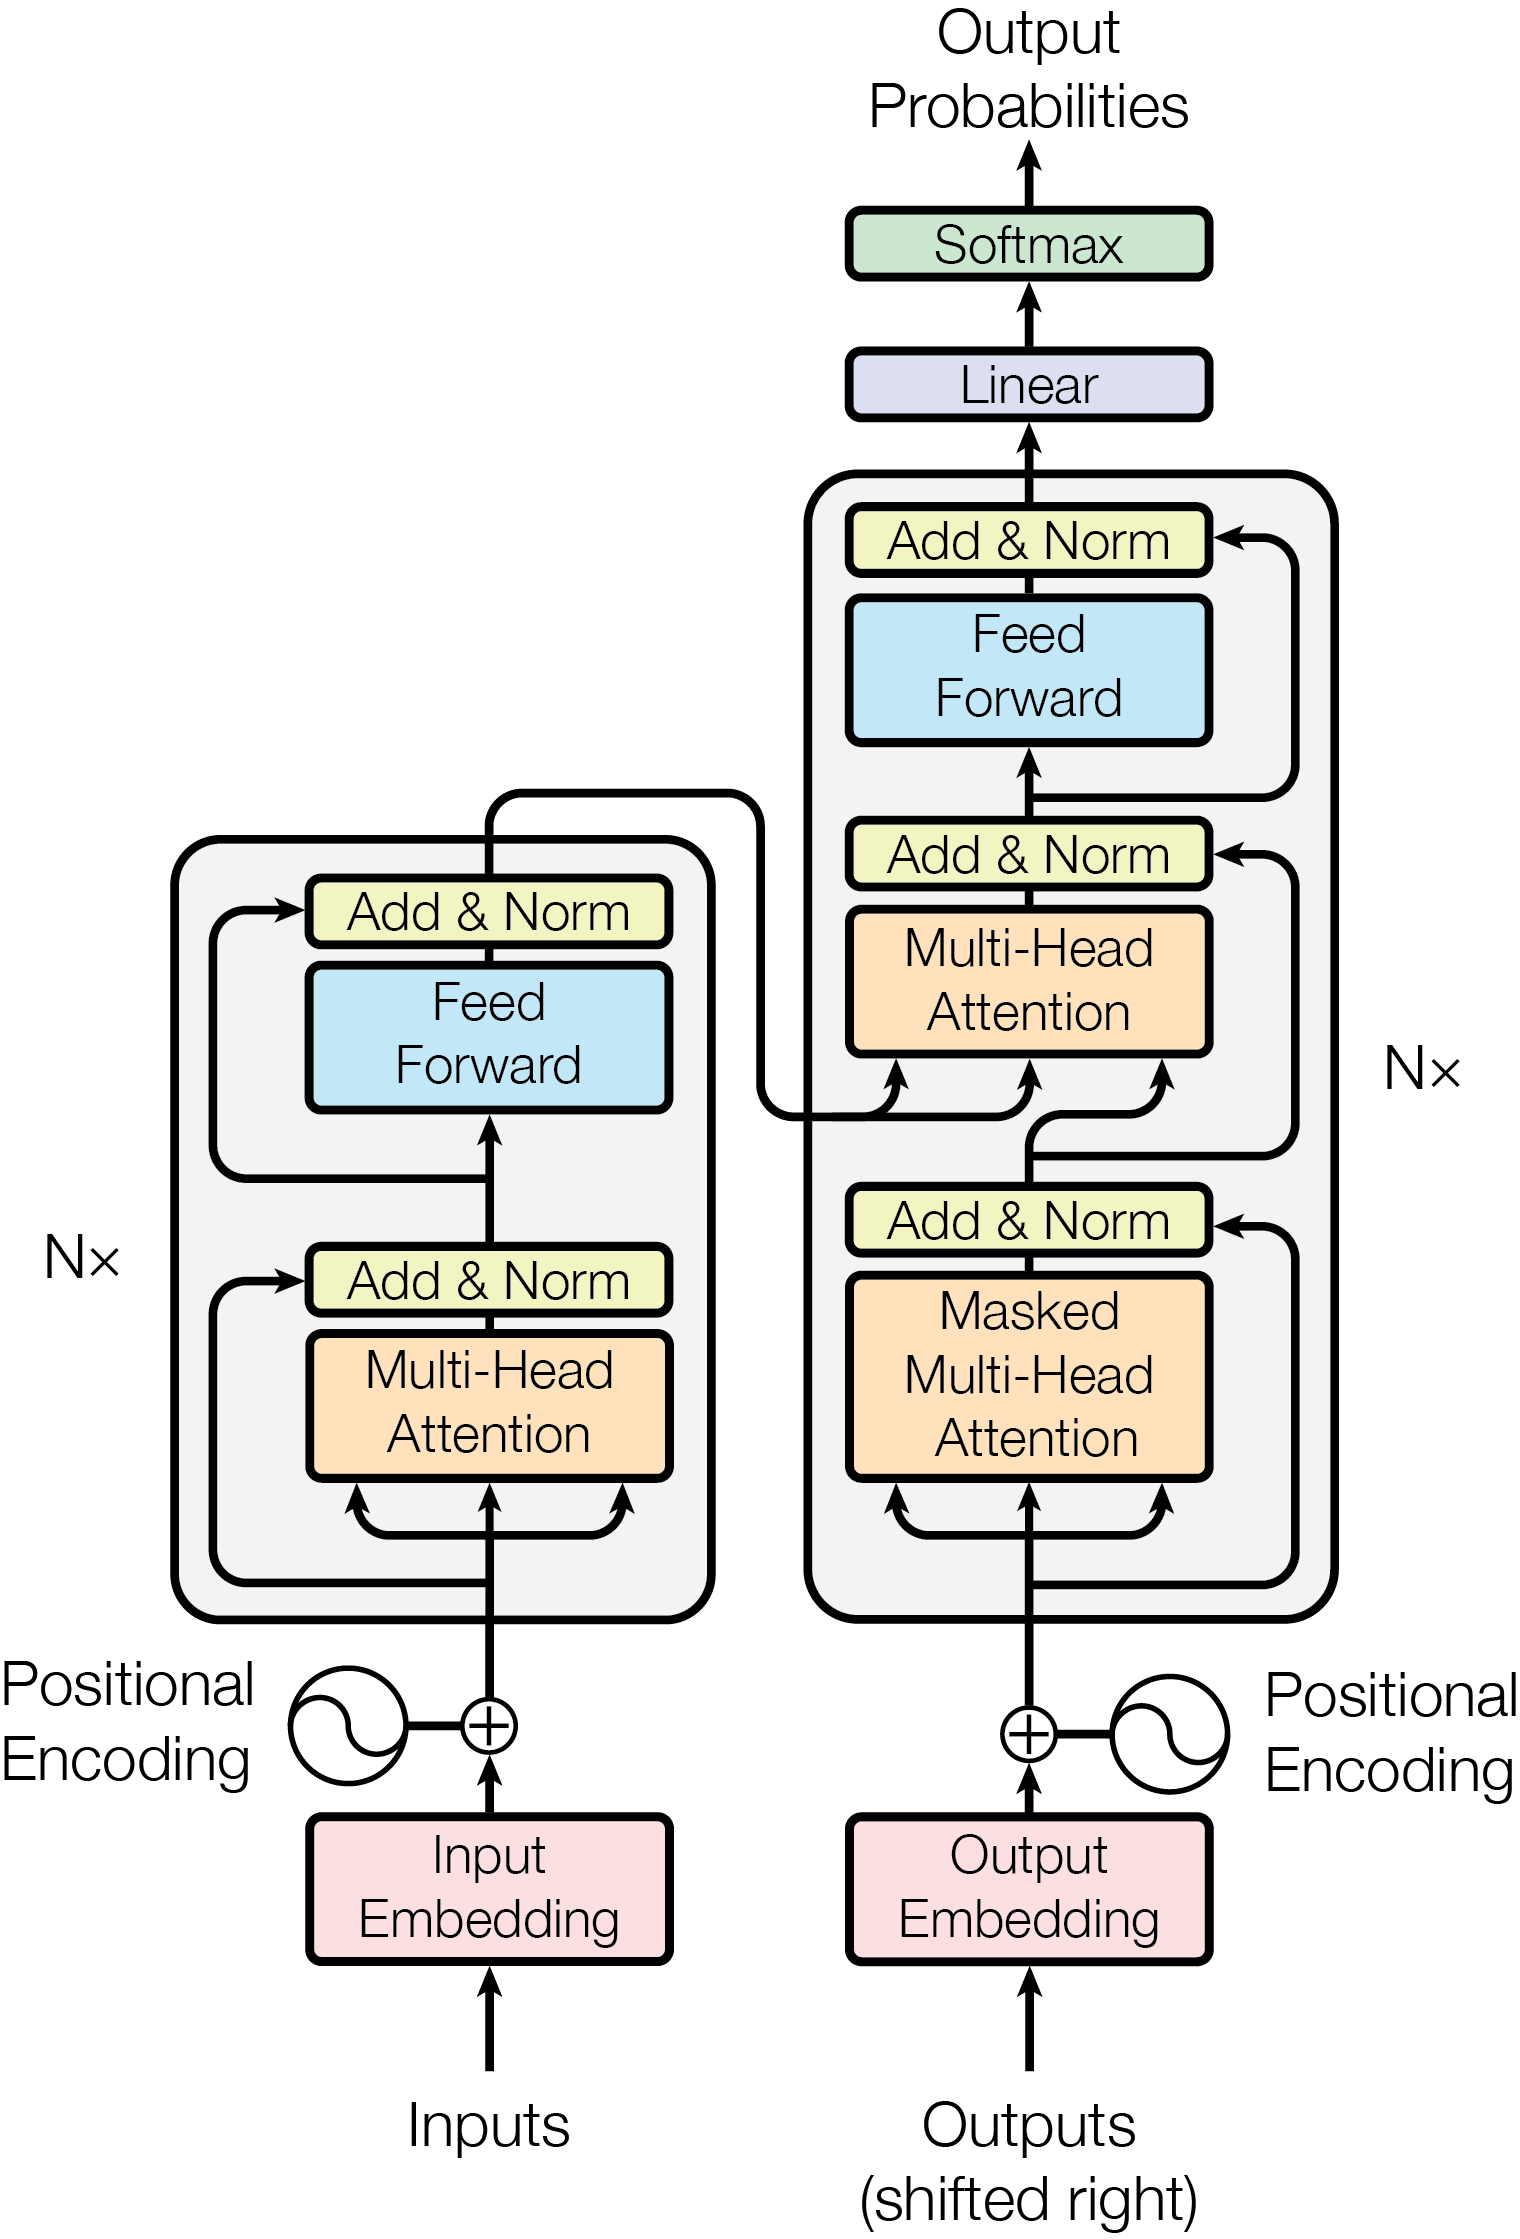
\includegraphics[scale=0.20]{figs/architecture.png}
	\caption{Schemat blokowy architektury transformera}
	\label{fig:transformer_architecture}
\end{figure}

\section{Zasada działania}
Działanie transformera opiera się na mechanizmie tzw. self-attention oraz na omówionych warstwach kodujących i dekodujących.
W ramach mechanizmu self-attention wykonywane są dwie główne operacje zwane scaled dot-product attention oraz multi-head attention.

\subsection{Scaled dot-product}
Scaled dot-product attention to działanie polegające na obliczeniu wag dla poszczególnych wartości, tym samym określa, jak bardzo dane fragmenty sekwencji są ze sobą powiązane.
Sekwencja wejściowa jest dzielona odpowiednio na wektory K (klucze), Q (zapytania) o długości $d_{k}$ i V (wartości) o długości $d_{v}$.
Następnie wykonuje się iloczyn skalarny pomiędzy kluczami i zapytaniami, który dzieli się przez pierwiastek z $d_{k}$.
Na koniec obliczana jest funkcja softmax w celu obliczenia wag. 
W praktyce macierz wyników obliczana jest na macierzach kluczy, wartosci i zapytań jak pokazano we wzorze \ref{eq:attention}.  

\begin{equation}
    \text{Attention}(Q, K, V) = \text{softmax}\left(\frac{Q K^T}{\sqrt{d_k}}\right) V
    \label{eq:attention}
\end{equation}
% Przykładowe równanie to
% \begin{equation}
%     E = m c^2
%     \label{eq:Emc2},
% \end{equation}
% gdzie $E$ oznacza \dots\
    
Jak podkreślają autorzy, czynnik czynnik faktoryzujący $\frac{1}{d_{k}}$ przyczynia się do zwiększenia szybkości i jest bardziej efektywny pod względem wykorzystania pamięci, ze względu na możliwość wykorzystania zoptymalizowanych algorytmów wykonujących obliczenia na macierzach.
Rozwiązanie to zostało zaproponowane w kontrze do istniejącej już funkcji uwagi zwanej additive attention. 
 
\subsection{Multi-Head Attention}
Proces ten polega na liniowej projekcji zapytań, kluczy i wartości $h$ razy.
Każdy z poszczególnych elementów jest rzutowany na mniejsze przestrzenie za pomocą $h$ różnych, uczonych projekcji liniowych, dzięki czemu uzyskuje się wymiar $d_{k}$ dla kluczy i zapytań oraz $d_{v}$ dla wartości.
Następnie dla każdej z tych zredukowanych projekcji równolegle wykonywana jest funkcja uwagi co skutkuje uzyskaniem na wyjściu wektora o wymiarze $d_{v}$.
Po zakończeniu obliczeń przez poszczególne głowy ich wyniki łączone są w jeden wektor co zostało pokazane we wzorze \ref{eq:multiheadattention}.

\begin{equation} \label{eq:multiheadattention}
    \text{MultiHead}(Q, K, V) = \text{Concat}\left( \text{head}_{1} \text{,} \text{...} \text{,} \text{head}_{h} \right) W^{O}
\end{equation}

Takie podejście sprawia, że model w procesie uczenia jest w stanie jednoczesnie analizować informacje z różnych podprzestrzeni reprezentacji przy zachowaniu podobnego kosztu obliczeniowego, jak w przypadku pojedycznej uwagi.
% Działanie transformera opiera się na warstwie kodującej oraz na warstwie dekodującej.
% Zadaniem warstwy kodującej jest zakodowanie argumentów wejściowych (np. tekstu, obrazów) do postaci numerycznej. 
% Warstwa dekodująca, wykorzystuje przekazane z warstwy kodującej zakodowane informacje do przetworzenia ich na wartości wyjściowe (np. do tekstu czy wideo). \\
